\documentclass[krantz1,ChapterTOCs]{krantz}
\usepackage{fixltx2e,fix-cm}
\usepackage{amssymb}
\usepackage{amsmath}
\usepackage{graphicx}
\usepackage{subfigure}
\usepackage{makeidx}
\usepackage{multicol}
\usepackage{qrcode}

 
% \usepackage[dvips]{hyperref}

\usepackage{tikz}
\usepackage{xcolor}
\usetikzlibrary{scopes}
\usepackage{verbatim} 
\usetikzlibrary{patterns}
\usepackage{algorithm}
\usepackage{algpseudocode}
\usepackage{listings}
	\definecolor{codegreen}{rgb}{0,0.6,0}
	\definecolor{codegray}{rgb}{0.5,0.5,0.5}
	\definecolor{codepurple}{rgb}{0.58,0,0.82}
	\definecolor{backcolour}{rgb}{0.92,0.92,0.92}
	\lstset{language=Python, 
	backgroundcolor=\color{backcolour},   
	commentstyle=\color{codegreen},
	keywordstyle=\color{magenta},
	numberstyle=\tiny\color{codegray},
	stringstyle=\color{codepurple},
	basicstyle=\fontsize{8}{11}\ttfamily,
	frame=lines,
%	numbers=left,
	tabsize=2,
	morekeywords={models, lambda, forms}}


\frenchspacing
\tolerance=5000

\makeindex

\newtheorem{theorem}{Teorema}
\newtheorem{exercise}{Exercício}[chapter]
\newtheorem{example}{Exemplo}
\newtheorem{definition}{Definição}
\newtheorem{proof}{Prova}
 %place custom commands and macros here

\begin{document}

\frontmatter

\title{Robótica Móvel 
%in Socio-Environmental Systems, Public Health, and Insurance\\
%{\Large(Applied Environmental Statistics Series)}
}
\author{Jeferson J. Lima}

\maketitle

%\cleardoublepage
\thispagestyle{empty}
\vspace*{\stretch{1}}
\begin{center}
\Large\itshape
To my dog\\
and my cat.
\end{center}
\vspace{\stretch{2}}
%\cleardoublepage
\setcounter{page}{7} %previous pages will be reserved for frontmatter to be added in later.
\tableofcontents
%\chapter*{Foreword}
I am delighted to introduce the first book on Multimedia Data Mining.  When I came to know about this book project undertaken by two of the most active young researchers in the field, I was pleased that this book is coming in early stage of a field that will need it more than most fields do.  In most emerging research fields, a book can play a significant role in bringing some maturity to the field.  Research fields advance through research papers.  In research papers, however, only a limited perspective could be provided about the field, its application potential, and the techniques required and already developed in the field.  A book gives such a chance.  I liked the idea that there will be a book that will try to unify the field by bringing in disparate topics already available in several papers that are not easy to find and understand.  I was supportive of this book project even before I had seen any material on it.  The project was a brilliant and a bold idea by two active researchers.  Now that I have it on my screen, it appears to be even a better idea.  

Multimedia started gaining recognition in 1990s as a field.  Processing, storage, communication, and capture and display technologies had advanced enough that researchers and technologists started building approaches to combine information in multiple types of signals such as audio, images, video, and  text.  Multimedia computing and communication techniques recognize correlated information in multiple sources as well as insufficiency of information in any individual source.    By properly selecting sources to provide complementary information, such systems aspire, much like human perception system, to create a holistic picture of a situation using only partial information from separate sources.

Data mining is a direct outgrowth of progress in data storage and processing speeds.  When it became possible to store large volume of data and run different statistical computations to explore all possible and even unlikely correlations among data, the field of data mining was born.  Data mining allowed people to hypothesize relationships among data entities and explore support for those.  This field has been put to applications in many diverse domains and keeps getting more applications.  In fact many new fields are direct outgrowth of data mining and it is likely to become a powerful computational tool.\vadjust{\vfill\pagebreak}



%\chapter*{Preface}
Approximately 17 million people in the USA (6{\%} of the
population) and 140 million people worldwide (this number is
expected to rise to almost 300 million by the year 2025) suffer
from \textit{diabetes mellitus}. Currently, there a few dozens of
commercialised devices for detecting blood glucose levels [1].
However, most of them are invasive. The development of a
noninvasive method would considerably improve the quality of life
for diabetic patients, facilitate their compliance for glucose
monitoring, and reduce complications and mortality associated with
this disease. Noninvasive and continuous monitoring of glucose
concentration in blood and tissues is one of the most challenging
and exciting applications of optics in medicine. The major
difficulty in development and clinical application of optical
noninvasive blood glucose sensors is associated with very low
signal produced by glucose molecules. This results in low
sensitivity and specificity of glucose monitoring by optical
methods and needs a lot of efforts to overcome this difficulty.

A wide range of optical technologies have been designed in
attempts to develop robust noninvasive methods for glucose
sensing. The methods include infrared absorption, near-infrared
scattering, Raman, fluorescent, and thermal gradient
spectroscopies, as well as polarimetric, polarization
heterodyning, photonic crystal, optoacoustic, optothermal, and
optical coherence tomography (OCT) techniques [1-31].

For example, the polarimetric quantification of glucose is based
on the phenomenon of optical rotatory dispersion, whereby a chiral
molecule in an aqueous solution rotates the plane of linearly
polarized light passing through the solution. The angle of
rotation depends linearly on the concentration of the chiral
species, the pathlength through the sample, and the molecule
specific rotation. However, polarization sensitive optical
technique makes it difficult to measure \textit{in vivo} glucose
concentration in blood through the skin because of the strong
light scattering which causes light depolarization. For this
reason, the anterior chamber of the eye has been suggested as a
sight well suited for polarimetric measurements, since scattering
in the eye is generally very low compared to that in other
tissues, and a high correlation exists between the glucose in the
blood and in the aqueous humor. The high accuracy of anterior eye
chamber measurements is also due to the low concentration of
optically active aqueous proteins within the aqueous humor.

On the other hand, the concept of noninvasive blood glucose
sensing using the scattering properties of blood and tissues as an
alternative to spectral absorption and polarization methods for
monitoring of physiological glucose concentrations in diabetic
patients has been under intensive discussion for the last decade.
Many of the considered  effects, such as changing of the size,
refractive index, packing, and aggregation of RBC under glucose
variation, are important for glucose monitoring in diabetic
patients. Indeed, at physiological concentrations of glucose,
ranging from 40 to 400 mg/dl, the role of some of the effects may
be modified, and some other effects, such as glucose penetration
inside the RBC and the followed hemoglobin glycation, may be
important [30-32].

Noninvasive determination of glucose was attempted using light
scattering of skin tissue components measured by a
spatially-resolved diffuse reflectance or NIR fre\-quen\-cy-domain
reflectance techniques. Both approaches are based on change in
glucose concentration, which affects the refractive index mismatch
between the interstitial fluid and tissue fibers, and hence
reduces scattering coefficient. A glucose clamp experiment showed
that reduced scattering coefficient measured in the visible range
qualitatively tracked changes in blood glucose concentration for
the volunteer with diabetes studied.




\listoffigures
\listoftables
%%%\twocolumn
\chapter*{Contributors}

\begin{multicols}{2}
\contributor{Michael Aftosmis}{NASA Ames Research Center}{Moffett Field, California}

\contributor{Pratul K. Agarwal}{Oak Ridge National Laboratory}{Oak Ridge, Tennessee}

\contributor{Sadaf R. Alam}{Oak Ridge National Laboratory}{Oak Ridge, Tennessee}

\contributor{Gabrielle Allen}{Louisiana State University}{Baton Rouge, Louisiana}

\contributor{Martin Sandve Aln{\ae}s}{Simula Research Laboratory and University of Oslo, Norway}{Norway}

\contributor{Steven F. Ashby} {Lawrence Livermore National Laboratory}{Livermore, California}

\contributor{David A. Bader} {Georgia Institute of Technology}{Atlanta, Georgia}

\contributor{Benjamin Bergen} {Los Alamos National Laboratory}{Los Alamos, New Mexico}

\contributor{Jonathan W. Berry} {Sandia National Laboratories}{Albuquerque, New Mexico}

\contributor{Martin Berzins}{University of Utah}{Salt Lake City, Utah}

\contributor{Abhinav Bhatele}{University of Illinois}{Urbana-Champaign, Illinois}

\contributor{Christian Bischof} {RWTH Aachen University}{Germany}

\contributor{Rupak Biswas} {NASA Ames Research Center}{Moffett Field, California}\vspace*{5pt}

\contributor{Eric Bohm} {University of Illinois}{Urbana-Champaign, Illinois}\vspace*{5pt}

\contributor{James Bordner} {University of California, San Diego}{San Diego, California}\vspace*{5pt}

\contributor{George Bosilca} {University of Tennessee}{Knoxville, Tennessee}\vspace*{5pt}

\contributor{Greg L. Bryan} {Columbia University}{New York, New York}\vspace*{5pt}

\contributor{Marian Bubak} {AGH University of Science and Technology}{
Krak{\'o}w, Poland}\vspace*{5pt}

\contributor{Andrew Canning}{Lawrence Berkeley National
Laboratory}{Berkeley, California}

\contributor{Jonathan Carter} {Lawrence Berkeley National
Laboratory}{Berkeley, California}

\contributor{Zizhong Chen} {Jacksonville State University}{Jacksonville,
Alabama}

\contributor{Joseph R. Crobak} {Rutgers, The State University of New
Jersey}{Piscataway, New Jersey}

\contributor{Roxana E. Diaconescu} {Yahoo! Inc.}{Burbank, California}

\contributor{Peter Diener}
{Louisiana State University}{Baton Rouge, Louisiana}

\contributor{Jack J. Dongarra} {University of Tennessee, Knoxville, 
Oak Ridge National Laboratory, and}{University of Manchester}

\contributor{John B. Drake} {Oak Ridge National Laboratory}{Oak Ridge,
Tennessee}

\contributor{Kelvin K. Droegemeier} {University of Oklahoma}{Norman,
Oklahoma}

\contributor{St{\'e}phane Ethier} {Princeton University}{Princeton, New
Jersey}

\contributor{Christoph Freundl}
{Friedrich--Alexander--Universit{\"a}t}{Erlangen, Germany}

\contributor{Karl F{\"u}rlinger} {University of Tennessee}{Knoxville,
Tennessee}

\contributor{Al Geist} {Oak Ridge National Laboratory}{Oak Ridge,
Tennessee}

\contributor{Michael Gerndt} {Technische Universit{\"a}t
M{\"u}nchen}{Munich, Germany}

\contributor{Tom Goodale}
{Louisiana State University}{Baton Rouge, Louisiana}

\contributor{Tobias Gradl}
{Friedrich--Alexander--Universit{\"a}t}{Erlangen, Germany}

\contributor{William D. Gropp} {Argonne National Laboratory}{Argonne,
Illinois}

\contributor{Robert Harkness} {University of California, San
Diego}{San Diego, California}

\contributor{Albert Hartono} {Ohio State University}{Columbus, Ohio}

\contributor{Thomas C. Henderson} {University of Utah}{Salt Lake City,
Utah}

\contributor{Bruce A. Hendrickson} {Sandia National
Laboratories}{Albuquerque, New Mexico}

\contributor{Alfons G. Hoekstra} {University of Amsterdam}{Amsterdam,
The Netherlands}

\contributor{Philip W. Jones} {Los Alamos National Laboratory}{Los
Alamos, New Mexico}

\contributor{Laxmikant Kal{\'e}} {University of
Illinois}{Urbana-Champaign, Illinois}

\contributor{Shoaib Kamil} {Lawrence Berkeley National
Laboratory}{Berkeley, California}

\contributor{Cetin Kiris} {NASA Ames Research Center}{Moffett Field,
California}

\contributor{Uwe K{\"u}ster} {University of Stuttgart}{Stuttgart,
Germany}

\contributor{Julien Langou} {University of Colorado}{Denver, Colorado}

\contributor{Hans Petter Langtangen}
{Simula Research Laboratory and}{University of Oslo, Norway}

\contributor{Michael Lijewski} {Lawrence Berkeley National
Laboratory}{Berkeley, California}

\contributor{Anders Logg}
{Simula Research Laboratory and}{University of Oslo, Norway}

\contributor{Justin Luitjens} {University of Utah}{Salt Lake City, Utah}

\contributor{Kamesh Madduri} {Georgia Institute of Technology}{Atlanta,
Georgia}

\contributor{Kent-Andre Mardal}
{Simula Research Laboratory and}{University of Oslo, Norway}

\contributor{Satoshi Matsuoka} {Tokyo Institute of Technology}{Tokyo,
Japan}

\contributor{John M. May} {Lawrence Livermore National
Laboratory}{Livermore, California}

\contributor{Celso L. Mendes} {University of Illinois}{Urbana-Champaign,
Illinois}

\contributor{Dieter an Mey} {RWTH Aachen University}{Germany}

\contributor{Tetsu Narumi} {Keio University}{Japan}

\contributor{Michael L. Norman} {University of California, San
Diego}{San Diego, California}

\contributor{Boyana Norris} {Argonne National Laboratory}{Argonne,
Illinois}

\contributor{Yousuke Ohno} {Institute of Physical and Chemical Research
(RIKEN)}{Kanagawa, Japan}

\contributor{Leonid Oliker} {Lawrence Berkeley National
Laboratory}{Berkeley, California}

\contributor{Brian O'Shea} {Los Alamos National Laboratory}{Los Alamos,
New Mexico}

\contributor{Christian D. Ott}
{University of Arizona}{Tucson, Arizona}

\contributor{James C. Phillips} {University of
Illinois}{Urbana-Champaign, Illinois}

\contributor{Simon Portegies Zwart} {University of
Amsterdam,}{Amsterdam, The Netherlands}

\contributor{Thomas Radke}
{Albert-Einstein-Institut}{Golm, Germany}

\contributor{Michael Resch} {University of Stuttgart}{Stuttgart,
Germany}

\contributor{Daniel Reynolds} {University of California, San Diego}{San
Diego, California}

\contributor{Ulrich R{\"u}de}
{Friedrich--Alexander--Universit{\"a}t}{Erlangen, Germany}

\contributor{Samuel Sarholz}
{RWTH Aachen University}{Germany}

\contributor{Erik Schnetter}
{Louisiana State University}{Baton Rouge, Louisiana}

\contributor{Klaus Schulten} {University of Illinois}{Urbana-Champaign,
Illinois}

\contributor{Edward Seidel}
{Louisiana State University}{Baton Rouge, Louisiana}

\contributor{John Shalf} {Lawrence Berkeley National
Laboratory}{Berkeley, California}

\contributor{Bo-Wen Shen} {NASA Goddard Space Flight Center}{Greenbelt,
Maryland}

\contributor{Ola Skavhaug}
{Simula Research Laboratory and}{University of Oslo, Norway}

\contributor{Peter M.A. Sloot} {University of Amsterdam}{Amsterdam, The
Netherlands}

\contributor{Erich Strohmaier} {Lawrence Berkeley National
Laboratory}{Berkeley, California}

\contributor{Makoto Taiji} {Institute of Physical and Chemical Research
(RIKEN)}{Kanagawa, Japan}

\contributor{Christian Terboven}
{RWTH Aachen University,}{Germany}

\contributor{Mariana Vertenstein} {National Center for Atmospheric
Research}{Boulder, Colorado}

\contributor{Rick Wagner} {University of California, San Diego}{San
Diego, California}

\contributor{Daniel Weber} {University of Oklahoma}{Norman, Oklahoma}

\contributor{James B. White, III} {Oak Ridge National Laboratory}{Oak
Ridge, Tennessee}

\contributor{Terry Wilmarth} {University of Illinois}{Urbana-Champaign,
Illinois}

\end{multicols}
%\chapter*{Symbols}
\begin{symbollist}{000000}
\symbolentry{$\alpha$}{To solve the generator maintenance scheduling, in the  past, several mathematical techniques have  been applied.}
\symbolentry{$\sigma^2$}{These include integer programming, integer linear programming, dynamic programming, branch and bound etc.}
\symbolentry{$\sum$}{Several heuristic search algorithms have also been developed. In recent years expert systems,}
\symbolentry{$abc$}{fuzzy approaches, simulated annealing and genetic algorithms have also been tested.}
\symbolentry{$\theta\sqrt{abc}$}{This paper presents a survey of the literature}
\symbolentry{$\zeta$}{ over the past fifteen years in the generator}
\symbolentry{$\partial$}{maintenance scheduling. The objective is to}
\symbolentry{sdf}{present a clear picture of the available recent literature}
\symbolentry{ewq}{of the problem, the constraints and the other aspects of}
\symbolentry{bvcn}{the generator maintenance schedule.}
\end{symbollist}

\mainmatter


\part{Introdução a Robótica Móvel}
\chapterauthor{Jeferson J. Lima}{Departamento de Informática (DAINF) \\Universidade Tecnológica Federal do Paraná (UTFPR)}

\chapter{Introdução a Robótica Móvel}

% \section{Introdução}\label{intro-ch0}

% \section{Introdução}\label{intro}

% A component part for an electronic item is
% manufactured at one of three different factories, and then delivered to
% the main assembly line.Of the total number supplied, factory A supplies
% 50\%, factory B 30\%, and factory C 20\%. Of the components
% manufactured at factory A, 1\% are faulty and the corresponding
% proportions for factories B and C are 4\% and 2\% respectively. A
% component is picked at random from the assembly line. What is the
% probability that it is faulty?

\section{Primeiros passos com a Linguagem Python}\label{python}

É comum quando estamos iniciando no mundo da matemática, nos depararmos com a necessidade de desenhar gráficos, algo como a figura baixo:

\begin{figure}
    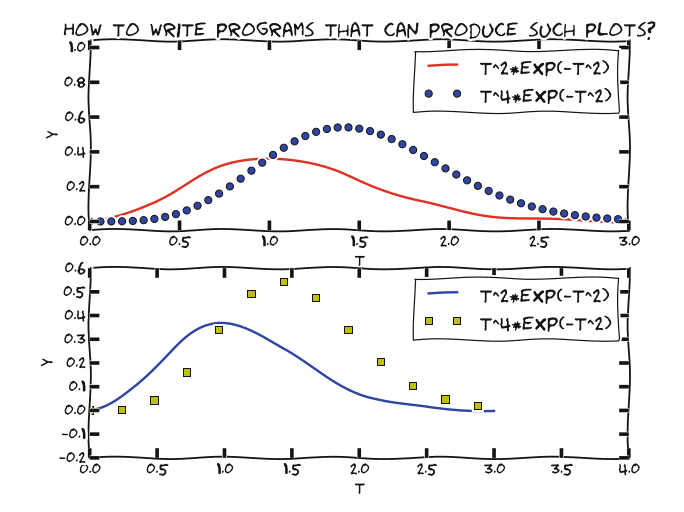
\includegraphics[width=200pt]{chapters/chapter0/figures/manual_graph.png}
    \caption[Desenhando Gráficos Manualmente]{Desenhando Gráficos Manualmente}
\end{figure}

Não somente nas engenharia os profissionais necessitam das habilidades de manipular e exibi-los dados graficamente,
a maioria das pessoas tem experiencias em softwares como Microsoft Excel, Libreoffice Calc, entre outras ferramentas dedicadas.
No entanto, essa interação geralmente é bastante simples, com alguns cliques é possível gerar diversos gráficos para visualização dos dados.

Porém, dada a característica dos dados a serem plotados, faz-se necessário um nível de customização maior, surgindo a necessidade.

Python é uma excelente linguagem para iniciantes, bem como usuários avançados, pois possui uma sintaxe simples e clara. Outro ponto
forte é as bibliotecas de python que apresenta diversas opções para processamento e visualização de dados. Destaca-se inicialmente aqui, duas
bibliotecas que serão utilizadas no inicialmente, a biblioteca para processamento numérico \textbf{numpy}, biblioteca \textbf{scipy} com diversas
funções da área de ciência da computação e \textbf{matplotlib} para visualização dos dados.
\subsection{Instalação do Python}

Para estudar desta matéria, você precisa de uma instalação do Python que atenda ao propósito de aula. A maneira mais rápida de obter uma instalação útil do Python em seu computador Windows ou Mac,
é baixar e instalar o Anaconda (https://www.anaconda.com/). Em muitas distribuições de linux, o Python já é nativo,
caso não seja, aconselha-se a instalação pelo terminal utilizando linha de comando.

\begin{lstlisting}
    $ sudo apt-get install python3
\end{lstlisting}

A versão de Python2 está obsoleta desde janeiro de 2020, sendo assim, nem suporte desde então. Por este motivo aconselha-se
a instalação de Python3.

A instalação de uma biblioteca do Python pode ser dada através do comando:
\begin{lstlisting}
    $ sudo python3 -m pip install numpy
\end{lstlisting}

Há diversas opções de serviços online, como a ferramenta Colab do Google, onde disponibiliza opções com recursos computacionais interessantes,
a uma conta google são oferecidas três opções de hardware, Máquina sem GPU, com GPU e uma Máquina com TPU.

\subsection{Problemas Numéricos com Python}

Para o nosso primeiro exemplo de problema numérico utilizando a linguagem Python, vamos fazer uso da expressão do grafico abaixo.

\begin{equation*}
    y = t^2\exp(-t^2)
\end{equation*}

Neste momento, teremos que recorrer a algumas funções da biblioteca \textbf{numpy}, como \textbf{numpy.exp} e \textbf{numpy.linspace} para gerar um vetor de tempo $t$.

\begin{lstlisting}
    ## importando bibliotecas
    from numpy import exp, linspace
    ## Definindo a funcao
    def yf(t):
        return t**2*exp(-t**2)

    # vetor t, inicio em 0 e fim em 3
    #   com 50 elementos
    t = linspace(0,3,50)

    y = yf(t)
\end{lstlisting}

Assim a variável $y$ recebe $y_f(t)$.

\subsubsection{Plotando Dados}

Dando continuidade ao exemplo anterior, apresentamos aqui outra biblioteca do python, a  \textbf{matplotlib} para visualização dos dados.
Considerando o exemplo acima, temos:

\begin{lstlisting}
    ## importando bibliotecas
    from numpy import exp, linspace
    ## Definindo a funcao
    def yf(t,n):
        return t**n*exp(-t**2)

    # vetor t, inicio em 0 e fim em 3
    #   com 50 elementos
    t = linspace(0,3,50)

    y1 = yf(t,2)
    y2 = yf(t,4)

    # importando o modulo pyplot e renomeando como plt
    import matplotlib.pyplot as plt

    plt.plot(t,y1)
    plt.plot(t,y2, "o")
    plt.xlabel("t")
    plt.ylable("y")
    plt.legend(["T^2*EXP(-T^2)", "T^4*EXP(-T^2)"])
\end{lstlisting}

O resultado esperado será:

\begin{figure}[htb]
    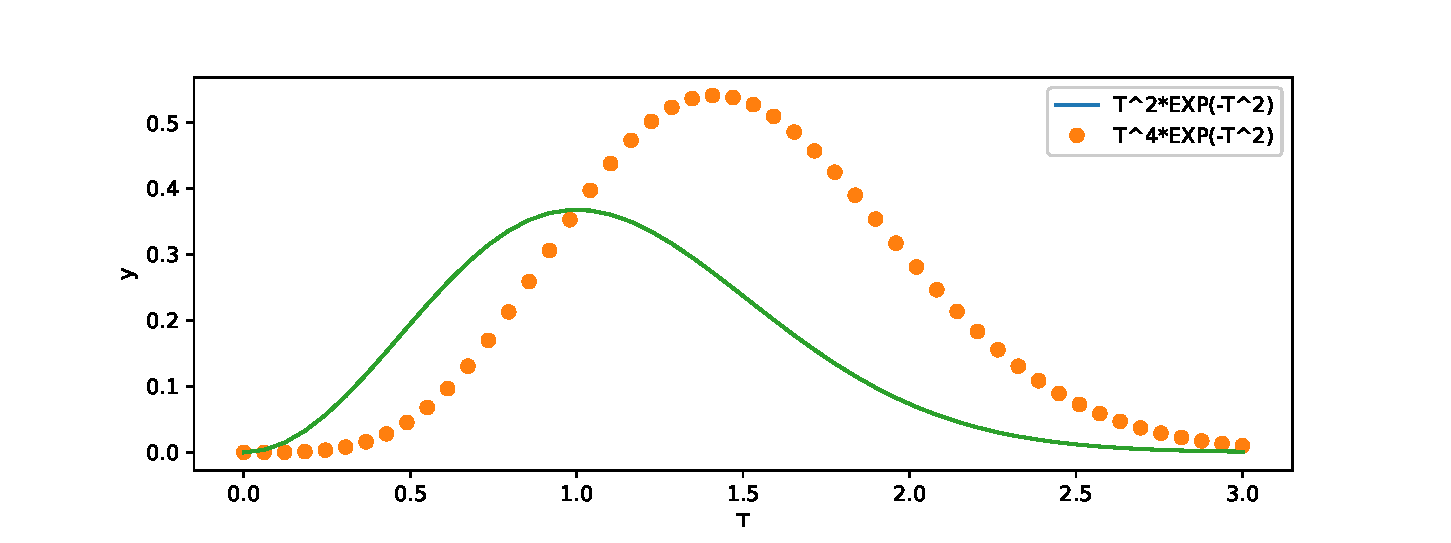
\includegraphics[width=300pt]{chapters/chapter0/figures/python_graph.eps}
    \caption[Desenhando Gráficos Manualmente]{Matplotlib Gráficos}
\end{figure}

A uma série de customizações que podem ser feitas no gráfico, como escrever a legenda em latex, mudança de cores, etc ... Para mais informações consulte a documentação do 
\textbf{matplotlib} na internet.

\subsubsection{Simulação numérica de Sistemas Dinâmicos}

\begin{VF}
    ``Um sistema dinâmico contínuo é um sistema dinâmico cujo estado evolui ao longo do espaço de estado continuamente de acordo com uma regra fixa.''
    
    \VA{Jaime E. Villate}{Introdução aos sistemas dinâmicos, 2007}
    \end{VF}

    Para entender melhor como resolver numericamente um sistemas dinâmicos utilizando uma linguagem de programação, primeiro precisamos recorrer ao problema.

    Aqui será apresentado um problema simples, onde deseja se saber a velocidade de um veículo, considerando limitações impostas pelo seu modelo dinâmico, O veículo está sobre uma superfície plana em condições de rolagem... então é aplicado uma força de tração $u$ ("um empurrão") no sentido do seu movimento, $b$ será o coeficiente de atrito e $m$ a massa.

\begin{figure}[htb]
    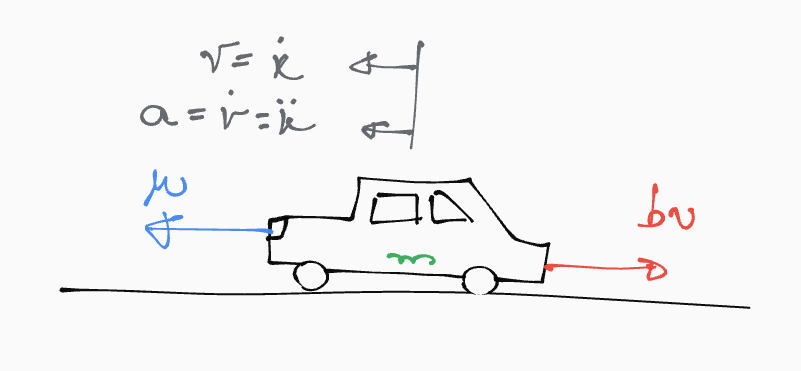
\includegraphics[width=300pt]{chapters/chapter0/figures/cruise_control_schematic.png}
    \caption[Desenhando Gráficos Manualmente]{Matplotlib Gráficos}
\end{figure}

Deve-se agora listar as forças com base na física do sistema.

\begin{equation*}
    m\dot{v}+bv=u
\end{equation*}

Substituindo $v$ por $\dot{x}$:

\begin{equation*}
    m\ddot{x}+b\dot{x}=u
\end{equation*}

sendo $x$, posicionamento, $\dot{x}$ velocidade e $\ddot{x}$ aceleração, temos então a função de espaço de estados:

\begin{equation}\label{eq:car}
    \frac{d}{dt}\begin{bmatrix} x_0 \\ x_1 \end{bmatrix} = 
    \begin{bmatrix} 1 & 0\\ -\displaystyle\frac{b}{m} & +\displaystyle\frac{1}{m} \end{bmatrix}
    \begin{bmatrix} x_1 \\ u \end{bmatrix}    
\end{equation}

A solução numérica de Eq. \ref{eq:car} é obtida através de um método de integração, em Python a biblioteca \textbf{scipy} traz os diversos métodos de integração, a função responsável por chamar o integrador é \textbf{odeint}.

\begin{lstlisting}
    import numpy as np
    import matplotlib.pyplot as plt
    from scipy.integrate import odeint

    ## Definindo a funcao carro
    def car(x,t):
        m = 2000
        b = 240
        u = 100
        # inicializando vetor derivadas
        dx = np.zeros(2,)
        dx[0] = x[1]
        dx[1] = 1/m*(-b*x[1]+u)
        return dx

    # vetor t, inicio em 0 e fim em 3
    #   com 100 elementos
    t = np.linspace(0,10,100)
    # condicoes iniciais
    x0 = [0,0]

    # integrador
    x = odeint(car, x0, t)

    # plotando os valores
    plt.plot(t,x[:,0],t,x[:,1])
    plt.xlabel("t")
    plt.legend(["Posicao", "Velocidade"]) 
\end{lstlisting}
 
A solução numérica pode ser vista pelo gráfico abaixo:

\begin{figure}[htb]
    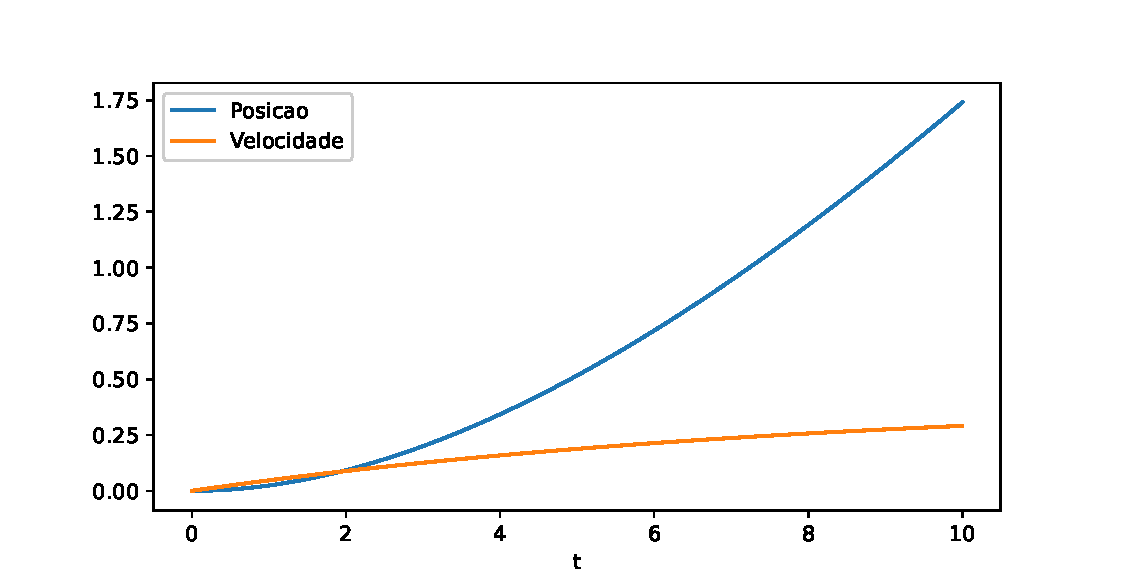
\includegraphics[width=300pt]{chapters/chapter0/figures/exercice_car.eps}
    \caption[Modelo Dinâmico Carro]{Gráfico velocidade e Posicionamento Carro}
\end{figure}

O sistema apresentado possui apenas dois estados, no entanto, sistemas de maior ordem podem ser
simulados utilizando os métodos de integração, como será visto no próximo capítulo.

\begin{shortbox}
    \Boxhead{Exercício de Fixação}
    Com base no sistema do robô demonstrado acima, escreva um programa que simule a situação onde o robô é inicializado em uma rampa com angulo de $\theta=30$ graus, lembre que ele sob da força gravitacional $G=\sin(\theta)mg$, onde $m$ é a massa e $g$ é a
    força gravitacional. Qual vai ser a velocidade e posicionamento final do robô após decorrido 10 segundos. Parâmetros: Força de tração $u=8\text{Nm}$,
    coeficiente de atrito $b=2$ e massa $m=3$.
    \begin{center}
        Resposta:

        \qrcode[height=0.5in]{Posicionamento, Velocidade: -2.0704, -0.2.432}
\end{center}

\end{shortbox}

\subsubsection{Biblioteca Simbólica}

Em algumas situações, faz se interessante utilizar ferramentas para facilitar e/ou simplificar a solução de sistemas de equações. Neste caso utilizaremos a biblioteca \textbf{sympy}, que possui várias ferramentas para solução de equações dinâmicas.

Vamos a um exemplo:

\begin{lstlisting}
    from sympy import *

    # definindo x como uma variavel
    x = symbols('x')
    eq = (sin(x)**2 + cos(x)**)**2

    # expandir equacao eq
    expand(eq)
    # >> sin(x)**4 + 2*sin(x)**2*cos(x)**2 + cos(x)**4

    # simplificar equacao eq
    simplify(eq)
    # >> 1

\end{lstlisting}

Para memorizar o uso da ferramenta de solução de equações simbólicas, vamos a alguns exercícios de fixação.

\begin{shortbox}
    \Boxhead{Exercício de Fixação}
    \begin{enumerate}
        \item  Usando o função \textbf{solve(eq,x)} encontre a solução da função quadrática $ax^2+bx+c=0$.
        \begin{center}
            Solução:

\qrcode[height=1in]{
x = symbols('x')
a = symbols('a')
b = symbols('b')
c = symbols('c')
eq2 = a*x**2+b*x+c
solve(eq2, x)
# >>[(-b + sqrt(-4*a*c + b**2))/(2*a), -(b + sqrt(-4*a*c + b**2))/(2*a)]}
\end{center}

    \item Sendo $x(t)$ uma função no tempo, use o comando \textbf{x = Function('x')} para definir a função $x$ e $t$ como 
    uma variável simbólica. Como o comando \textbf{dsolve(eq, x(t))} ache a solução da equação $\displaystyle\frac{dx(t)}{dt}+x(t)=0$
    \begin{center}
        Solução:

\qrcode[height=1in]{
x = Function('x')
t = symbols('t')
eq = diff(x(t), t) + x(t)
dsolve(eq, x(t))
eq2 = a*x**2+b*x+c
dsolve(eq2, x)
# >>Eq(x(t), C1*exp(-t))}
\end{center}

\end{enumerate}
\end{shortbox}



\section{Glossário}
\begin{Glossary}
\item[360 Degree Review] Performance review that includes feedback from superiors, peers, subordinates, and clients.
% \item[Abnormal Variation] Changes in process performance that cannot be accounted for by typical day-to-day variation. Also referred to as
% non-random variation.
% \item[Acceptable Quality Level (AQL)] The minimum number of parts that must comply with quality standards, usually stated as a percentage.
% \item[Activity] The tasks performed to change inputs into outputs.
% \item[Adaptable] An adaptable process is designed to maintain effectiveness and efficiency as requirements change. The process is
% deemed adaptable when there is agreement among suppliers, owners, and customers that the process will meet
% requirements throughout the strategic period.
\end{Glossary}





\part{Cinemática e Dinâmica de Robôs Móveis}
\chapterauthor{Jeferson J. Lima}{Departamento de Informática (DAINF) \\Universidade Tecnológica Federal do Paraná (UTFPR)}
\chapter{Cinemática e Dinâmica de Robôs Móveis com Rodas}


\section{Introdução}\label{intro}
% 2. Cinemática e Dinâmica de Robôs Móveis com Rodas
% 	2.1 Cinemática Direta e Inversa
% 		2.1.1 Cinemática Direta e Inversa
% 		2.1.1 Cinemática de Robôs Móveis com Rodas
% 	2.2 Restrições de Movimento
% 		2.2.1 Sistemas Holonômicos
% 		2.2.2 Sistemas Não-Holonômicos
% 	2.3 Modelagem de Robô Móvel com restrições de Movimento.
% 3. Controle Moderno para Robótica Móvel
% 	3.1 Lyapunov-based Controle
% 	3.2 SDRE Controle
% 4. Eventos Não Deterministicos em Robótica Móvel
% 	4.1 Estimação de Estados
% 	4.2 Filtro Bayesiano
% 	4.3 Filtro de Kalman
% 		4.3.1 Filtro de Kalman Estendido

A humanidade é fascinada pelo movimento das rodas a milhares de anos, isso intriga até os dias de hoje, o homem moderno.
Na matemática há áreas específicas para descrever o movimento dos corpos, ou para o nosso interesse nesse capítulo, a cinemática dos robôs. 
Um modelo cinemático de um robô, com rodas ou pernas, descreve as relações geométricas entre que dão forma ao próposito deste robô.

Em resumo, os modelos cinemáticos estão relacionadas a como as velocidades dos elementos do robô interagem entre si e o espaço.

\section{Rotação, Translação e Transformação Homogênea}\label{rotacao}
 
Para representação de posicionamento e orientação de um sistema de coordenadas faz se necessário seguir a metodologia do sistema universal de coordenadas.

De acordo com \cite{craig2009introduction} uma vez estabelecido o sistema de coordenada como um vetor de posição $\mathbb{R}^{3 \times 1}$, composto pelas coordenadas $X,Y$ e $Z$, podemos então representar os operadores de rotação, translação e transformação homogênea como operações matriciais. Desta forma, um ponto ${}^A\mathbf{P}$ representa a distância ao longo dos eixos do plano $\{A\}$. Os elementos individuais de ${}^A\mathbf{P}$ podem ser visto pela equação \eqref{eq:cine1}.

\begin{equation}\label{eq:cine1}
    {}^A\mathbf{P} = \begin{bmatrix}
    p_x\\ p_y \\ p_z
    \end{bmatrix}.
    \end{equation}
    
    A representação gráfica de ${}^A\mathbf{P}$ pode ser vista na figura \ref{fig:cine1f}. 
    
    \begin{figure}[!ht]
    \centering
    \begin{tikzpicture}[scale=0.8]
    \node(p0) at (0,0){};
    \draw [->] (p0.center) --++(0,3) node[right] {$ Y_A$};
    \draw [->, rotate =120] (p0.center) --++(0,3) node[below] {$ Z_A$};
    \draw [->, rotate =240] (p0.center) --++(0,3) node[below] {$ X_A$};
    \draw [->] (p0.center) --++(2.5,0.5) node(B)[above,rotate=30] {${}^A\mathbf{P}$};
    \node at (-1.5,2.5) {$\{A\}$};
    \end{tikzpicture}
    \caption{Vetor em relação ao plano $\{A\}$}
    \label{fig:cine1f}
    \end{figure}
    
    Além da definição das coordenadas de um vetor, torna-se necessário definir a orientação desse corpo no espaço. O vetor definido por ${}^A\mathbf{P}$ pode ser rotacionado pela matriz de rotação $\mathbf{R}$, conforme a equação \eqref{eq:cine2}.
    
    \begin{equation}\label{eq:cine2}
    {}_A^B
    \mathbf{R} = 
    \begin{bmatrix}
    r_{11} & r_{11} & r_{11}\\
    r_{21} & r_{21} & r_{21}\\
    r_{31} & r_{31} & r_{31}\\
    \end{bmatrix}
    \end{equation}


    Na figura abaixo, a posição de ${}^A\mathbf{P}$ (sistema de referência global) em relação a ${}^B\mathbf{P}$ é encontrado através da multiplicação da matriz de ${}_B^A \mathbf{R}(\theta)$ (lê-se rotação do sistema de referência $B$ em $A$) pela posição de ${}^B\mathbf{P}$

    \begin{figure}[!ht]
        \centering
        \begin{tikzpicture}[scale=0.8]
            \node(p0) at (0,0){};
            \draw [->] (p0.center) --++(0,3) node[right] {$\hat Y_A$};
            \draw [->, rotate =120] (p0.center) --++(0,3) node[below] {$\hat Z_A$};
            \draw [->, rotate =240] (p0.center) --++(0,3) node[below] {$\hat X_A$};
            \draw [->, rotate =-10, gray] (p0.center) --++(1.5,2) node(A)[above,rotate=30] {${}^A\mathbf{P}$};
            \node(p1) at (6,1){};
            \draw [->, rotate =30, red] (p0.center) --++(0,3) node[right,rotate=30] {$\hat Y_B$};
            \draw [->, rotate =150, red] (p0.center) --++(0,3) node[below,rotate=30] {$\hat Z_B$};
            \draw [->, rotate =270, red] (p0.center) --++(0,3) node[below,rotate=30] {$\hat X_B$};
            \draw [->, rotate =20, red] (p0.center) --++(1.5,2) node(B)[above,rotate=30] {${}^B\mathbf{P}$};
        \end{tikzpicture}
        \caption{Vetor em rotação no plano $\{A\}$}
        \label{fig:vetor_rot}
    \end{figure}
    
    Abaixo segue um exercício numérico de fixação.

    \begin{shortbox}
        \Boxhead{Exercício de Fixação}
        Como exemplo, uma rotação $\theta$ de ${}^AP$ em torno do eixo $Z$ é descrita pela figura  \eqref{fig:vetor_rot}. 
        
        
        
        Pode-se observar que é adicionado uma coluna e linhas com zeros e uma nova linha em  \eqref{eq:cine3}, essa notação torna-se necessária pois será posteriormente apresentando o operador de translação.

        \begin{equation}\label{eq:cine3}
        {}^B\mathcal{P} = {}_A^B \mathbf{R}(\theta) {}^A\mathbf{P} = 
        \begin{bmatrix}
        \cos(\theta) & \sin(\theta) & 0 & 0\\
        \sin(\theta) & \cos(\theta) & 0 & 0\\
        0 & 0 & 1 & 0\\ 
        0 & 0 & 0 & 1\\
        \end{bmatrix}.
        \begin{bmatrix}
        {}^Ap_x\\
        {}^Ap_y\\
        {}^Ap_z\\
        1
        \end{bmatrix}
        \end{equation}
        \begin{center}
            Resposta:
    
\qrcode[height=0.8in]{
[-1,  0,  0,  0],
[ 0, -1,  0,  0],
[ 0,  0,  1,  0],
[ 0,  0,  0,  1]]
}
    \end{center}
    
    \end{shortbox}

    A rotação pode acontecer tanto em $x, y$ ou $z$, conforme é mostrado abaixo:

    \begin{equation*}
        \mathbf{R}_x(\theta) =
        \begin{bmatrix}
            1 & 0            & 0             \\
            0 & \cos(\theta) & -\sin(\theta) \\
            0 & \sin(\theta) & \cos(\theta)  \\
        \end{bmatrix} \text{, eixo $x$ fixo}
    \end{equation*}
    \begin{equation*}
        \mathbf{R}_y(\theta) =
        \begin{bmatrix}
            \cos(\theta)  & 0 & \sin(\theta) \\
            0             & 1 & 0            \\
            -\sin(\theta) & 0 & \cos(\theta) \\
        \end{bmatrix} \text{, eixo $y$ fixo}
    \end{equation*}
    \begin{equation*}
        \mathbf{R}_z(\theta) =
        \begin{bmatrix}
            \cos(\theta) & -\sin(\theta) & 0 \\
            \sin(\theta) & \cos(\theta) & 0 \\
            0            & 0            & 1 \\
        \end{bmatrix} \text{, eixo $z$ fixo}
    \end{equation*}

    Frequentemente o sistema de referência $\{A\}$ não coincide em nenhum coordenada de $\{B\}$, sendo assim, deve-se representar o deslocamento entre os planos. Esse deslocamento é chamado de translação, e dá-se pelo operador translacional $\mathbf{D}_A(q)$, onde ${}^A\mathbf{Q}$ representa uma translação entre os planos $\{A\}$ e $\{B\}$ e é expresso pela equação \eqref{eq:cine4}.

    \begin{equation}\label{eq:cine4}
    {}^A\mathbf{Q} =
    \begin{bmatrix}
    q_x\\ q_y \\ q_z
    \end{bmatrix}, \qquad \mathrm{e} \qquad
    \mathbf{D}_A = 
    \begin{bmatrix}
    1 & 0 & 0 & q_x\\
    0 & 1 & 0 & q_y\\
    0 & 0 & 1 & q_z\\
    0 & 0 & 0 & 1
    \end{bmatrix}.
    \end{equation}
    
    Adota-se agora a notação para translação e rotação de um vetor, conforme a equação \eqref{eq:cine5}. Observa-se que a matriz $\mathbf{D}_A$ foi incorporada pela nova notação.
    
    \begin{equation}\label{eq:cine5}
    \begin{bmatrix}
    {}^B_A\mathbf{P}\\ 1
    \end{bmatrix}
    =
    \underbrace {
    \left[
    \begin{matrix}
    & {}_B^A\mathbf{R}& \\ \hline
    0 & 0 & 0\\
    \end{matrix} \right.
    \left.
    \vline
    \begin{matrix}
    {}^A\mathbf{Q}\\ \hline
    1
    \end{matrix} \right]
    }_{{}^A_B\mathcal{A}}
    \begin{bmatrix}
    {}^B\mathbf{P}\\
    1
    \end{bmatrix}
    \end{equation}
    
    
    Na equação \eqref{eq:cine5} a matriz ${}^A_B\mathcal{A}$ representa a matriz de transformação homogênea, neste caso, composta pela matriz de rotação ${}^A_B \mathbf{R}$ e de translação ${}^A\mathbf{Q}$. Pode-se ver graficamente o resultado da operação da equação \eqref{eq:cine5} pela figura \ref{fig:cine2}
    
    \begin{figure}[!ht]
    \centering
    \begin{tikzpicture}
    \node(p0) at (0,0){};
    \draw [->] (p0.center) --++(0,3) node[right] {$\hat Y_A$};
    \draw [->, rotate =120] (p0.center) --++(0,3) node[below] {$\hat Z_A$};
    \draw [->, rotate =240] (p0.center) --++(0,3) node[below] {$\hat X_A$};
    \draw [->, dotted] (p0.center) --++(1.5,4) node(B)[above,rotate=30] {${}^B\mathbf{P}$};
    \node(p1) at (6,1){};
    \draw [->, rotate =30] (p1.center) --++(0,3) node[right,rotate=30] {$\hat Y_B$};
    \draw [->, rotate =150] (p1.center) --++(0,3) node[below,rotate=30] {$\hat Z_B$};
    \draw [->, rotate =270] (p1.center) --++(0,3) node[below,rotate=30] {$\hat X_B$};
    \draw [->] (p1.center) --++(1.5,4) node(B)[above,rotate=30] {${}^B\mathbf{P}$};
    \draw [dotted,-latex] (p0)  -- (p1) node[midway, fill=white]{${}^A\mathbf{Q}$};
    \draw [-latex,dashed] (p0)  -- (B);
    \node at (-1.5,2.5) {$\{A\}$};
    \node at (4,2.5)  [rotate=30]   {$\{B\}$};
    \end{tikzpicture}
    \caption{Transformação homogênea do ponto ${}^AP$ pelos operadores de rotação e translação}
    \label{fig:cine2}
    \end{figure}
    
    Na forma generalizada, a transformação homogênea ${}^{i}_0\mathbf{T}$ pode ser expressa por uma sucessiva pode ser encontrada fazendo o produto das sucessivas transformações de ${}^{i-1}_0\mathcal{A}_i$. Conforme é mostrado na equação \eqref{fig:cine3}.
    
    \begin{equation}\label{fig:cine3}
    \begin{array}{lcl}
    {}^i_0\mathbf{T} &= & {}^0_1\mathcal{A}{}^1_2\mathcal{A} \cdots {}^{i-1}_i\mathcal{A} = \prod \limits^i_{j=1}{}^{j-1}_i\mathcal{A}, \quad \mathrm{para\;}i=1,2,\cdots,n\\[.2cm]
    & = &
    \begin{bmatrix}
    x_i & y_i & z_i & p_i\\
    0 & 0 & 0 & 1
    \end{bmatrix} = 
    \begin{bmatrix}
    {}^i_0\mathbf{R} & {}^i_0\mathcal{P}\\
    \mathbf{0} & 1
    \end{bmatrix}
    \end{array}
    \end{equation}
    
    \noindent onde, ${}^i_0\mathcal{P}$ é o vetor de orientação do referencial $i$ em relação a base $0$.


\section{Cinemática Direta e Inversa}\label{intro-ch1}

A Cinemática é a ciência que trata do movimento (geométrico) e das forças que o causam [Craig]. Desta forma, dependendo do ponto de visão,
podemos referênciar a cinemática de um robô através de uma referência externa (Cinemática externa), como por exemplo a relação entre o robô e
as coordenadas de um mapa global. Há a possibilidade também, da referência ser o próprio robô, desta forma da-se o nome de
Cinemática Interna, como exemplo, podemos citar a velocidade de rotação em torno do seu eixo ou velocidade das rodas.

Podemos ainda nos aprofundar mais sobre a Cinemática Interna do Robô, onde o espaço de ação das coordenadas definem a forma que se deve tratar o modelo de equações.
Considerando um robô fixo ou móvel com coordenadas generalizadas $\theta_1, \theta_2,..., \theta_n$ localizadas no espaço das \textcolor{red}{juntas ou atuadores (\textit{joint space}) $\mathbf{q}$}. Bem como $x_1, x_2,..., x_n$, o \textcolor{blue}{espaço das tarefas (\textit{task space}) $\mathbf{x}$}, temos então os vetores:

\begin{figure}[!ht]


\begin{tikzpicture}
    \newcommand{\nvar}[2]{%
    \newlength{#1}
    \setlength{#1}{#2}
    }

    % Define a few constants for drawing
    \nvar{\dg}{0.3cm}
    \def\dw{0.25}\def\dh{0.5}
    % Define commands for links, joints and such
    \def\link{\draw [double distance=1.5mm, very thick] (0,0)--}
    \def\joint{%
    \filldraw [fill=white] (0,0) circle (5pt);
    \fill[black] circle (2pt);
    }
    \def\grip{%
    \draw[ultra thick](0cm,\dg)--(0cm,-\dg);
    \fill (0cm, 0.5\dg)+(0cm,1.5pt) -- +(0.6\dg,0cm) -- +(0pt,-1.5pt);
    \fill (0cm, -0.5\dg)+(0cm,1.5pt) -- +(0.6\dg,0cm) -- +(0pt,-1.5pt);
    }

    \def\robotbase{%
    \draw[rounded corners=8pt] (-\dw,-\dh)-- (-\dw, 0) --
        (0,\dh)--(\dw,0)--(\dw,-\dh);
    \draw (-0.5,-\dh)-- (0.5,-\dh);
    \fill[pattern=north east lines] (-0.5,-1) rectangle (0.5,-\dh);
    }
    \newcommand{\doublelink}[6]{%
    \robotbase
    \link(#1:#2);
    \joint
    \begin{scope}[shift=(#1:#2), rotate=#1]
        \link(#3:#4);
        \joint
        \begin{scope}[shift=(#3:#4), rotate=#5]
            \grip
        \end{scope}
    \end{scope}
    }

    \doublelink{60}{2}{-90}{2}{-60}{1}
\end{tikzpicture}
    
\caption{Robô - Dois Graus de Liberdade}
\label{fig:2dof-robot}
\end{figure}

Assim sendo, da-se o nome de a \textcolor{red}{Cinemática Direta} quando o robô e descrito como função de entradas como (velocidade das rodas, movimento das juntas, direção das rodas).  Já a \textcolor{blue}{Cinemática Inversa} possibilita projetar um planejamento de movimento, o que significa que as entradas do robô podem ser calculadas para uma sequência de estado do robô desejada.

A relação entre as Cinemática Direta e Cinemática Inversa é obtida através da Matriz Jacobiana do Robô.

\begin{equation*}
    \mathbf{\dot{x}} = \mathbb{J}{\mathbf{\dot{q}}}
    \text{ e, }
    \mathbf{\dot{q}} = \mathbb{J}^{-1}{\mathbf{\dot{x}}}
\end{equation*}

bem como:

\begin{equation*}
    \frac{\text{d}\mathbf{x}}{\text{d}t} = \mathbb{J}\frac{\text{d}\mathbf{q}}{\text{d}t}
    \text{ e, }
    \frac{\text{d}\mathbf{q}}{\text{d}t} = \mathbb{J}^{-1}\frac{\text{d}\mathbf{x}}{\text{d}t}
\end{equation*}

onde $\mathbb{J}$ é dado por:
\begin{equation*}
    \mathbb{J}
    =
    \frac{d \mathbf{f}}{d \mathbf{q}}
    =
    \left[ \frac{\partial \mathbf{f}}{\partial q_1}
        \cdots \frac{\partial \mathbf{f}}{\partial q_n} \right]
    =
    \begin{bmatrix}
        \frac{\partial f_1}{\partial q_1} & \cdots &
        \frac{\partial f_1}{\partial q_n}                   \\
        \vdots                            & \ddots & \vdots \\
        \frac{\partial f_m}{\partial q_1} & \cdots &
        \frac{\partial f_m}{\partial q_n}
    \end{bmatrix}
\end{equation*}

Essa transformação é feita quando necessita-se, por exemplo, controlar um robô utilizando-se das referências de uma ferramenta acoplada a
extremidade do braço robótico. A Cinemática Inversa proporciona que a estratégia de controle seja aplicada na ferramenta até
que o objetivo da tarefa seja alcançado.


\begin{shortbox}
    \Boxhead{Exercício de Fixação}
    Levando em consideração o braço robótico da Figura \ref{fig:2dof-robot}, encontre as equações da cinemática do robô.
    \begin{equation*}
        \begin{split}
            x_f(t) = & l_1\cos(\theta_1)+l_2\cos(\theta_1 + \theta_2) \\            
            y_f(t) = & l_1\sin(\theta_1)+l_2\sin(\theta_1 + \theta_2)
        \end{split}
    \end{equation*}
    
    utilize a biblioteca \textbf{sympy} para solução do jacobiano.
    \begin{center}
        Resposta:

        \qrcode[height=0.5in]{https://ocw.mit.edu/courses/mechanical-engineering/2-12-introduction-to-robotics-fall-2005/lecture-notes/chapter5.pdf}
\end{center}

\end{shortbox} 


\section{Cinemática de Robôs Móveis com Rodas}

\subsection{Cinemática Biciclo}
\subsection{Cinemática Robô Diferencial}

\begin{figure}[!ht]
    \def\iangle{35} % Angle of the inclined plane
\def\down{0}
\def\arcr{0.7cm} % Radius of the arc used to indicate angles
\newcommand\centerofmass{%
    \tikz[radius=0.2em] {%
        \fill (0,0) -- ++(0.2em,0) arc [start angle=0,end angle=90] -- ++(0,-0.4em) arc [start angle=270, end angle=180];%
        \draw (0,0) circle;%
    }%
}

\begin{tikzpicture}[
    force/.style={>=latex,draw=blue,fill=blue},
    axis/.style={densely dashed,gray,font=\small},
    M/.style={rectangle,draw,fill=lightgray,minimum size=0.7cm,thin},
    m/.style={rectangle,draw=black,fill=lightgray,minimum size=0.3cm,thin},
    plane/.style={draw=black,fill=blue!10},
    string/.style={draw=red, thick},
    pulley/.style={thick},
    wheel/.style={fill=black, rounded corners=1.5pt},
]
     \begin{scope}[rotate=0]
        \node[M,transform shape] (M) at (-2,-1) {\centerofmass};
        % Draw axes and help lines
        {[axis,->]
            \draw (M) -- ++(0,2) node(y1_axis)[right] {$y'$};
        }
        % Forces
        {[force,->]
            % Assuming that Mg = 1. The normal force will therefore be cos(alpha)
            \draw (M.east) -- ++(1,0) node[above, blue] {$\mathbf{v}_{t-1}$};
        }
        \draw[wheel, fill=gray] (M.south west) rectangle ++(.4,-.1) node[]{};
        \draw[wheel, fill=gray] (M.north west) rectangle ++(.4,.1)  node[]{};
    \end{scope}


    %% Free body diagram of M
    \begin{scope}[rotate=\iangle]
        \node[M,transform shape] (M) {\centerofmass};
        % Draw axes and help lines
        {[axis,->]
            \draw (M) -- ++(0,2) node(y1_axis)[right] {$y'$};
            \draw (M) -- ++(2,0) node[right] {$x'$};
            % Indicate angle. The code is a bit awkward.
            \draw[solid,shorten >=0.5pt] (\down-\iangle:\arcr)
                arc(\down-\iangle:\down:\arcr);
            \node at (\down-0.5*\iangle:1.3*\arcr) {$\phi$};
        }
        % Forces
        {[force,->]
            % Assuming that Mg = 1. The normal force will therefore be cos(alpha)
            \draw (M.east) -- ++(1,0) node[above, blue] {$\mathbf{v}_t$};
        }
        \draw[wheel] (M.south west) rectangle ++(.4,-.1) node[below]{$v_D$};
        \draw[wheel] (M.north west) rectangle ++(.4,.1)  node[left]{$v_E$};
    \end{scope}
    % Draw gravity force. The code is put outside the rotated
    % scope for simplicity. No need to do any angle calculations. 
    \draw[axis,] (M.center) -- ++(1,0) node[below] {};
    %%
    \node[right, gray,font=\small, xshift=8] at (y1_axis) {$\{B\}$};
    %%
    \draw[, ->] (-2,-1) -- ++(4,0) node[below] {$x$};
    \draw[, ->] (-2,-1) -- ++(0,3) node(y_axis)[right] {$y$};
    \draw[gray, ->] (-2,-1) -- ++(-.5,-.5) node[left] {$z$};
    \node[left, gray,font=\small, xshift=-10] at (y_axis) {$\{A\}$};
\end{tikzpicture}

    \caption{Robô - Dois Graus de Liberdade}
    \label{fig:car01}
    \end{figure}

\subsection{Robô Omnidirecional}
\subsection{Robô Com Esteira}


\section{Dinâmica com Restrições de Movimento}

Tipicamente, um robô com rodas apresenta uma série de restrições relacionadas ao seu modelo de construção, tais restrição tem origem em limitações impostas pelas leis da cinemática e dinâmica.

As restrições dinâmicas têm origem proposta de modelo dinâmico do sistema, onde as limitação se apresentam devido a fatores como a inércia ou mesmo restrições nos atuadores \cite{klancar2017wheeled}.

Do lado da cinemática, as restrições estão relacionadas com a construção do robô e seu modelo cinemático. Podemos classificar as restrições cinemática, sendo elas holonômicas ou não holonômicas. Restrições holonômicas estão relacionadas a dimensionalidade da descrição do estado de um sistema, sendo ele expresso em coordenadas generalizadas, conforme demonstrado em Fig. \ref{fig:2dof-robot}.

Um sistema é considerado holonômico se não tiver restrições holonômicas, não apresentando assim, limitação em seu espaço de velocidades e portanto, todas as direções de movimento de espaço são possíveis. Neste aspecto, podemos considerar o Robô de dois graus de liberdade da Fig. \ref{fig:2dof-robot}, um sistema holonômico, caso não haja restrição da base do robô em $\theta_1$.

Já em um sistema não holonômico, tais restrições impedem que o robô, mova em direções arbitrárias. Um exemplo clássico é apresentado na Fig. \ref{fig:car01}, onde o robô diferencial possui restrições ao movimento em $y'$.




\subsection{Restrições Holonômicos}
 Um sistema holonômico possui restrições que dependem das coordenadas generalizadas, como já foi visto acima. Para tais sistemas com $n$ coordenadas generalizadas $\mathbf{q} = [q_1, \cdots, q_n]$, temos a seguinte equação que expressa tais restrições.

 \begin{equation}
     f(\mathbf{q}) = f(q_1, \cdots, q_n) = 0
     \label{eq:homo}
 \end{equation}

 onde a função $f$ e sua derivada são funções contínuas.

 Observa-se também que a função da equação Eq. \ref{eq:homo} não depende das velocidades ou de qualquer derivada de ordem superior com relação a $t$.

 Em geral, podemos ter $m$ restrições holonômicas, ou seja $(m<n)$.




 Equilíbrio de Energias - Formulação de Lagrange:

 \begin{equation}
     \mathcal{L}= \mathcal{T} - \mathcal{V}
 \end{equation}

A equação de energia cinética ($\mathcal{T}$) é dada por:

\begin{equation}
   \mathcal{T} = \frac{1}{2} \sum\limits_{k=1}^{N}{\mathbf{\dot{q}}_k}^T  \mathbf{M}_k {\mathbf{\dot{q}}_k}+ \frac{1}{2} \sum\limits_{k=1}^{N}\mathbf{\omega}_k^T \mathbf{J}_k \mathbf{\omega}_k
\end{equation}

A equação de Energia Potencial Gravitacional($\mathcal{V}_g$) é dada por\footnote{Depende do típo de energia potencial do sistema, neste caso - gravitacional}

\begin{equation}
   \mathcal{V}_g = \sum\limits_{k=1}^{N}\mathbf{M}g\Delta \underbrace{y_k}_{\text{altura}}
\end{equation}  


\begin{tabular}{l|l}
    $\mathbf{M}$               & Massa              \\
    $\mathbf{\omega}$ & Velocidade Angular \\
    $\mathbf{J}$               & Inércia         \\
\end{tabular}


Para Sistemas Holonômicos:
\begin{equation}
    \frac{d}{\df{t}}\left( \parcial{}{\mathcal{L}}{\dot{q}_k}\right)
    -\parcial{}{\mathcal{L}}{q_k}
    = f_k, \quad k = 1,2,...,n
\end{equation}


onde $k$ é o index das coordenadas generalizadas de $g_k$, $f_k$ são as forças externas que agem no sistema .

O modelo dinâmico de um robô movel sem restrições de movimento pode ser expresso pelo sistema de matrizes abaixo:

\begin{equation}
    \mathbf{M(q)\ddot{q}+ C(q, \dot{q})+ \color{red}{F(\dot{q})}\color{gray}+G(q) = E(q)u}
\end{equation}

onde, 
\begin{tabular}{ r | l }
  $\mathbf{q}$               & Vetor das coordenadas generalizadas   \\
  $\mathbf{M(q)}$            & Matriz de massa e inercia             \\
  $\mathbf{C(q, \dot{q})}$   & Vetor de força Coriolis e centrifuga  \\
  $\color{red}{\mathbf{F(\dot{q})}}$      & Vetor de atrito, força não conservativa\footnotemark\\
  $\mathbf{G(q)}$            & Vector da força gravitacional         \\
  $\mathbf{E(q)}$            & Matriz dos tranformação dos atuadores \\
  $\mathbf{u}$               & Vetor de entrada                      \\
\end{tabular}

\footnotetext{As forças que não fazem parte do balanço de energia no formalismo de lagrange, devem ser adicionadas a posteriori no sistema de equações}

A solução numérica pode ser dada através da integração da aceleração ($\mathbf{\ddot{q}}$):

\begin{equation}
    \mathbf{\ddot{q}}=\mathbf{M(q)}^{-1}\left\{\mathbf{-C(q, \dot{q})-F(\dot{q})-G(q) + E(q)u}\right\}
\end{equation}

Dito isso, usaremos o exemplo do braço robótico da Fig. \ref{fig:2dof-robot} para exrpressar o sistema em equações de estado, conforme a código abaixo:

\begin{equation*}
    \mathbf{X} = 
    \begin{bmatrix}
        \mathbf{q_1 q_2, \dot{q}_1, \dot{q}_2}.  
    \end{bmatrix}
\end{equation*}

\begin{lstlisting}[language=Python]
    def robot2dof(t,X):
        q1  = X[0]
        q2  = X[1]
        dq1 = X[2] 
        dq2 = X[3]
        # Inertial matrix
        Mq = np.array([...]) 
        # C Matrix
        Cq = np.array([...])
        # Gravitational matrix 
        Gq = np.array([...])
        # Friction Force
        ks = 0
        Fa = ks * np.array([[dq1],[dq1]])
        # Atuator
        U_gain =  tau1 = tau2 = 0
        Eu = U_gain * np.array([[tau1],[tau2]])
        # Init Model
        xdot = np.zeros(4,)
        
        #dinamic
        q2dot = inv(Mq).dot(-Cq-Fa-Gq)
        # states
        xdot[0] = dq1
        xdot[1] = dq2
        xdot[2] = q2dot[0]
        xdot[3] = q2dot[1]

        return xdot
\end{lstlisting}

\subsection{Sistemas Não-Holonômicos}


\section{Modelagem de Robô Móvel com restrições de Movimento}


\begin{figure}
    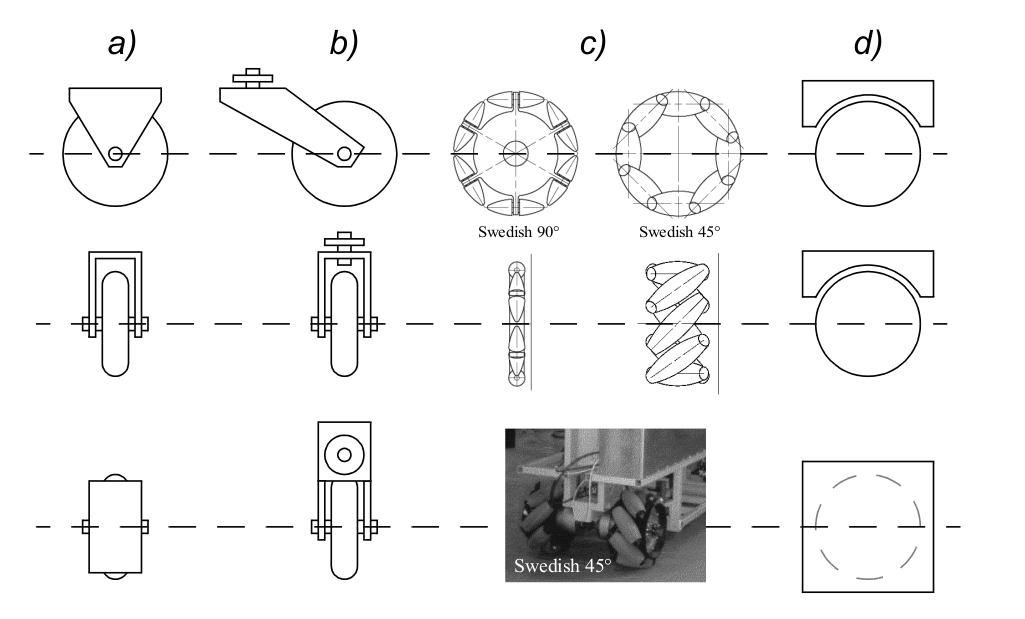
\includegraphics[width=0.8\textwidth]{chapters/chapter1/figures/tipo_de_rodas.png}
    % \cite{siegwart2011introduction}
    \caption{ (a) Standard wheel: two degrees of freedom. (b) castor wheel. (c) Swedish wheel: three degrees of freedom. (d) Ball or spherical wheel: realization technically difficult.}
\end{figure}


 Restrição não-holonômica

 O robô pode mover-se apenas na direção normal ao eixo das rodas motrizes


\begin{equation*}
    \dot{x}\sin(\phi) - \dot{y}\cos(\phi) = 0
\end{equation*}

As próprias rodas já inserem as restrições!


\begin{figure}
    \def\iangle{35} % Angle of the inclined plane
\def\down{0}
\def\arcr{0.7cm} % Radius of the arc used to indicate angles
\newcommand\centerofmass{%
    \tikz[radius=0.2em] {%
        \fill (0,0) -- ++(0.2em,0) arc [start angle=0,end angle=90] -- ++(0,-0.4em) arc [start angle=270, end angle=180];%
        \draw (0,0) circle;%
    }%
}

\begin{tikzpicture}[
    force/.style={>=latex,draw=blue,fill=blue},
    axis/.style={densely dashed,gray,font=\small},
    M/.style={rectangle,draw,fill=lightgray,minimum size=0.7cm,thin},
    m/.style={rectangle,draw=black,fill=lightgray,minimum size=0.3cm,thin},
    plane/.style={draw=black,fill=blue!10},
    string/.style={draw=red, thick},
    pulley/.style={thick},
    wheel/.style={fill=black, rounded corners=1.5pt},
]
     \begin{scope}[rotate=0]
        \node[M,transform shape] (M1) at (0,0) {\centerofmass};
        % Draw axes and help lines
        % Forces
        {[force,->]
            % Assuming that Mg = 1. The normal force will therefore be cos(alpha)
            \draw (M1.east) -- ++(1,0) node[above, blue] {$v$};
        }

        \draw[wheel,] (M1.south west) rectangle ++(.4,-.1) node[]{};
        \draw[wheel,] (M1.north west) rectangle ++(.4,.1)  node[]{};
    \end{scope}


    \begin{scope}[rotate=0]
        \node[M,transform shape] (M2) at (6,0) {\centerofmass};
        % Draw axes and help lines
        % Forces
        {[force,->]
            % Assuming that Mg = 1. The normal force will therefore be cos(alpha)
            \draw (M2.east) -- ++(1,0) node[above, blue] {$v$};
        }

        \draw[wheel,] (M2.south west) rectangle ++(.4,-.1) node[]{};
        \draw[wheel,] (M2.north west) rectangle ++(.4,.1)  node[]{};
    \end{scope}
    \begin{scope}[rotate=0]
        \node[M,transform shape] (M3) at (3,-2) {\centerofmass};
        % Draw axes and help lines
        % Forces
        {[force,->]
            % Assuming that Mg = 1. The normal force will therefore be cos(alpha)
            \draw (M3.center) -- ++(1,0) node[above, blue] {$v$};
            \draw (M3.center) -- ++(0,1) node[left, blue] {$v'$};
        }

        \draw[wheel,] (M3.south west) rectangle ++(.4,-.1) node[]{};
        \draw[wheel,] (M3.north west) rectangle ++(.4,.1)  node[]{};
    \end{scope}

%%
    \draw (-1,-1)           -- ++(2.5,0) node[](wall_1){};
    \draw (wall_1.center)   -- ++(0,-2) node[](wall_2){};
    \draw (wall_2.center)   -- ++(3.5,0) node[](wall_3){};
    \draw (wall_3.center)   -- ++(0,2) node[](wall_4){};
    \draw (wall_4.center)   -- ++(3,0) node[](wall_4){};    

    \pausar
    \draw[densely dashed, red] (M1.center) -- (M2.center);
    
    \pausar

    \begin{scope}[rotate=0]
        \node[M,transform shape] (M4) at (3,0) {\centerofmass};
        % Draw axes and help lines
        % Forces

        \draw[wheel,fill=gray] (M4.south west) rectangle ++(.4,-.1) node[]{};
        \draw[wheel,fill=gray] (M4.north west) rectangle ++(.4,.1)  node[]{};

        \draw[red] (3,0) -- ++(-0.6,-0.6) node[]{};
        \draw[red] (3,0) -- ++(0.6,-0.6) node[]{};
        \draw[red] (3,0) -- ++(-0.6,0.6) node[]{};
        \draw[red] (3,0) -- ++(0.6,0.6) node[]{};
    \end{scope}

    \draw[densely dashed, red] (M3.center) .. controls ++(1,0) and ++(-2,0) .. (M2.center);

    % Draw gravity force. The code is put outside the rotated
    % scope for simplicity. No need to do any angle calculations. 
\end{tikzpicture}

\end{figure}


\begin{figure}
    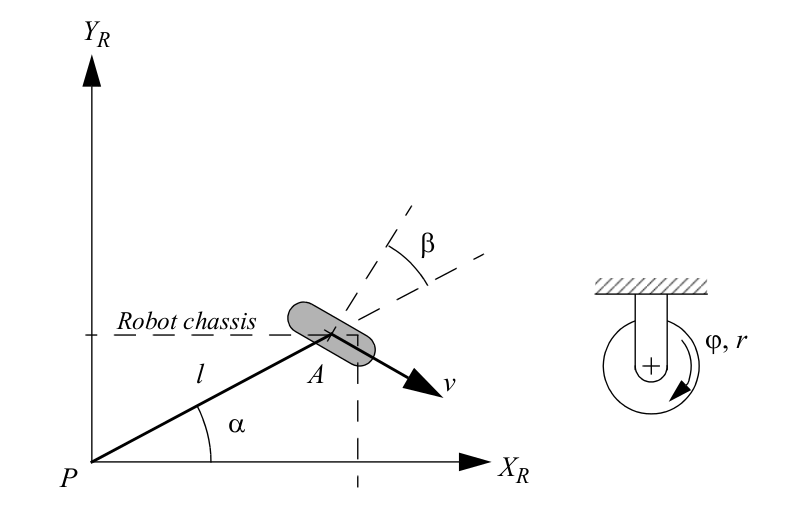
\includegraphics[width=0.6\textwidth]{chapters/chapter1/figures/wheels_const.png}    
    \caption{A fixed standard wheel and its parameters.}
\end{figure}










Restrições - Robô Diferencial

\def\iangle{35} % Angle of the inclined plane
\def\down{0}
\def\arcr{0.7cm} % Radius of the arc used to indicate angles
\newcommand\centerofmass{%
    \tikz[radius=0.2em] {%
        \fill (0,0) -- ++(0.2em,0) arc [start angle=0,end angle=90] -- ++(0,-0.4em) arc [start angle=270, end angle=180];%
        \draw (0,0) circle;%
    }%
}

\begin{tikzpicture}[
    force/.style={>=latex,draw=blue,fill=blue},
    axis/.style={densely dashed,gray,font=\small},
    M/.style={rectangle,draw,fill=lightgray,minimum size=0.7cm,thin},
    m/.style={rectangle,draw=black,fill=lightgray,minimum size=0.3cm,thin},
    plane/.style={draw=black,fill=blue!10},
    string/.style={draw=red, thick},
    pulley/.style={thick},
    wheel/.style={fill=black, rounded corners=1.5pt},
]
    %% Free body diagram of M
    \begin{scope}[rotate=\iangle]
        \node[M,transform shape] (M) {\centerofmass};
        % Draw axes and help lines
        {[axis,->]
            \draw (M) -- ++(0,1.3) node(y1_axis)[right] {$y$};
            \draw (M) -- ++(2,0) node[right] {$x$};
            % Indicate angle. The code is a bit awkward.
            \draw[solid,shorten >=0.5pt] (\down-\iangle:\arcr)
                arc(\down-\iangle:\down:\arcr);
            \node at (\down-0.5*\iangle:1.3*\arcr) {$\phi$};
        }
        % Forces
        {[force,->]
            % Assuming that Mg = 1. The normal force will therefore be cos(alpha)
            \draw (M.east) -- ++(1,0) node[above, blue] {$v_R$};
        }
        \draw[wheel] (M.south west) rectangle ++(.4,-.1) node[below]{$v_{D}$};
        \draw[wheel] (M.north west) rectangle ++(.4,.1)  node[left]{$v_{E}$};
        \draw [dotted, -](M) -- ++(0,2) node(CIR)[above] {CIR};
        \node[below,  yshift=-10, xshift=-5] at (CIR) {$\omega$};
    \end{scope}
    % Draw gravity force. The code is put outside the rotated
    % scope for simplicity. No need to do any angle calculations. 
    \draw[axis,] (M.center) -- ++(1,0) node[below] {};
    %%
    \node[right, gray,font=\small, xshift=8] at (y1_axis) {$\{R\}$};
    %%
    \draw[, ->] (-2,-1) -- ++(4,0) node[below] {$X$};
    \draw[, ->] (-2,-1) -- ++(0,3) node(y_axis)[right] {$Y$};
    \draw[gray, ->] (-2,-1) -- ++(-.5,-.5) node[left] {$Z$};
    \node[left, gray,font=\small, xshift=-10] at (y_axis) {$\{M\}$};
\end{tikzpicture}

\begin{equation}
    \mathbf{A} = 
    \begin{bmatrix}
        -\sin(\phi) & \cos(\phi) & 0
    \end{bmatrix}
\end{equation}


Equilíbrio de Energias:

\begin{equation}
    \mathcal{L}= \mathcal{T} - \mathcal{V}
\end{equation}

A equação de energia cinética ($\mathcal{T}$) é dada por:

\begin{equation}
    \mathcal{T} = \sum\limits_{i=0}^{N-1} \frac{1}{2} {}_{i}^{i+1}\dot{\mathbf{P}}^T\cdot m_{i}\cdot {}_{i}^{i+1}\dot{\mathbf{P}}+ \mathbf{\omega}_i^T\cdot \mathbf{J}_i \cdot \mathbf{\omega}_i
\end{equation}

ou para um robô em uma superfície:

\begin{equation*}
    \boxed{
        \mathcal{T} = \frac{m}{2}\left(\dot{x}^2+\dot{y}^2 \right)+ \frac{J}{2}\dot{\phi}^2}
    \text{, e  }
    \boxed{\mathcal{V} = 0}
\end{equation*}
               
    onde:
    \begin{tabular}{l|l}
        $m$               & Massa              \\
        $\mathbf{\omega}$ & Velocidade Angular \\
        $J$               & Inércia            \\
    \end{tabular}
              

Formulação de Lagrange

Para Sistemas Holonômicos:

\begin{equation}
    \frac{d}{\df{t}}\left( \parcial{}{\mathcal{L}}{\dot{q}_k}\right)
    -\parcial{}{\mathcal{L}}{q_k}
    +\tau_{d_k}
    = f_k, \quad k = 1,2,...,n
\end{equation}

Para Sistemas Não-Holonômicos \footnote{onde $k$ é o index das coordenadas generalizadas de $g_k$, $P$ representas as energias dissipativas (Atrito),
$\tau_d$ representa qualquer disturbio no sistema, $f_k$ são as forças externas que agem no sistema e $a_{jk}$ são os coeficientes das restrições de movimento.}
\begin{equation}
    \frac{d}{\df{t}}\left( \parcial{}{\mathcal{L}}{\dot{q}_k}\right)
    -\parcial{}{\mathcal{L}}{q_k}
    +\tau_{d_k}
    = f_k - \sum\limits^{m}_{j=1}\lambda_j a_{jk}
\end{equation}

O modelo dinâmico de um robô movel com restrições de movimento pode ser expresso pelo sistema de matrizes abaixo:

\begin{equation}
    \mathbf{M(q)\ddot{q}+ C(q, \dot{q})+ F(\dot{q})+G(q) = E(q)u -A}^T\mathbf{(q)}\boldsymbol{\lambda}
\end{equation}

onde:
\begin{tabular}{ r | l }
    $\mathbf{q}$               & Vetor das coordenadas generalizadas   \\
    $\mathbf{M(q)}$            & Matriz de massa e inercia             \\
    $\mathbf{C(q, \dot{q})}$   & Vetor de força Coriolis e centrifuga  \\
    $\mathbf{F(\dot{q})}$      & Vetor de atrito                       \\
    $\mathbf{G(q)}$            & Vector da força gravitacional         \\
    $\mathbf{E(q)}$            & Matriz dos tranformação dos atuadores \\
    $\mathbf{u}$               & Vetor de entrada                      \\
    $\mathbf{A}^T\mathbf{(q)}$ & Matriz de restrições de movimento     \\
    $\boldsymbol{\lambda}$     & Multiplicador de Lagrange             \\
\end{tabular}


A solução para $\lambda_i$ pode ser encontrada por:
\begin{itemize}
    \item Método 1: Pseudo-velocidades
    \item Método 2: Redução de Order 
    \item Método 3: Equações de Euler-Lagrange Modificadas 
    \item Método 4: Calculo das Forças de restrições 
\end{itemize}


Formulação de Lagrange - Pseudo-velocidades

O objetivo é resolver as restrições de $\lambda_i$:

\begin{equation}\label{eq:rmrestri}
    \mathbf{M(q)\ddot{q}+ C(q, \dot{q})+ F(\dot{q})+G(q) = E(q)u} - \textcolor{red}{\cancel{\mathbf{A}\mathbf{(q)}^T\boldsymbol{\lambda}}}
\end{equation}

reelembrando:

\begin{equation*}
    \mathbf{\dot{q}} = \mathbf{S}(q)\mathbf{v}
\end{equation*}

bem como:

\begin{equation}\label{eq:aprox_accel}
    \mathbf{\ddot{q}} = \mathbf{\dot{S}}(q)\mathbf{v} + \mathbf{S}(q)\mathbf{\dot{v}}
\end{equation}

Subustituindo \eqref{eq:rmrestri} em \eqref{eq:aprox_accel} e aplicando a relãção $\mathbf{A}(q)\mathbf{S}(q)=0$, temos a equação de aceleração do sistema:

\begin{equation}\label{eq:pseudovelo}
    \mathbf{\dot{v}} = \mathbf{\tilde{M}}^{-1}\left(\mathbf{\tilde{E}u - \tilde{V}} \right)
\end{equation}


Formulação de Lagrange - Pseudo-velocidades

\eqref{eq:pseudovelo} na forma de equação:

\begin{equation*}
    \mathbf{\dot{x}} =
    \begin{bmatrix}
        \mathbf{S}(q)\mathbf{v} \\
        \mathbf{-\tilde{M}}^{-1}\mathbf{\tilde{V}}
    \end{bmatrix}
    +
    \begin{bmatrix}
        \mathbf{0} \\
        \mathbf{\tilde{M}}^{-1}\mathbf{\tilde{E}}
    \end{bmatrix} \mathbf{u}
\end{equation*}

onde:

\begin{equation*}
    \begin{split}
        \mathbf{\tilde{V}} & =
        \mathbf{S}(q)^T\mathbf{M}\mathbf{\dot{S}}(q)\mathbf{v} + \mathbf{S}(q)^T (\mathbf{V + F + G})\\
        \mathbf{\tilde{M}} & = \mathbf{S}(q)^T\mathbf{M}\mathbf{S}(q)\\
        \mathbf{\tilde{E}} & = \mathbf{S}(q)^T\mathbf{E}\mathbf{S}
    \end{split}
\end{equation*}

onde:
\begin{tabular}{ r | l }
    $\mathbf{x}$ & Vetor de estados \\
    $\mathbf{S}$ & Matriz Jacobiana \\
\end{tabular}







% \section{Glossary}
% \begin{Glossary}
% \item[360 Degree Review] Performance review that includes feedback from superiors, peers, subordinates, and clients.
% \item[Abnormal Variation] Changes in process performance that cannot be accounted for by typical day-to-day variation. Also referred to as
% non-random variation.
% \item[Acceptable Quality Level (AQL)] The minimum number of parts that must comply with quality standards, usually stated as a percentage.
% \item[Activity] The tasks performed to change inputs into outputs.
% \item[Adaptable] An adaptable process is designed to maintain effectiveness and efficiency as requirements change. The process is
% deemed adaptable when there is agreement among suppliers, owners, and customers that the process will meet
% requirements throughout the strategic period.
% \end{Glossary}





% \part{Percepção e Ação}

% \part{Paradigmas de Controle}

% \part{Ambiente de Simulação}

% \part{Localização e Mapeamento Simultâneos}

% \part{Robôs Bípedes}

% \part{Robôs Aéreos}

\bibliographystyle{plain}
\bibliography{bibtex_example}

\printindex

\end{document}


% 1. Introdução a Robótica Móvel
% 	1.1 Primeiros Passos com a Linguagem Python
% 		1.1.1 Plotando Dados
% 		1.1.2 Simulação de Sistemas Dinâmicos
% 		1.1.3 Biblioteca simbólica
% 	1.2 Rotação, Translação e Transformação Homogênea
% 		1.2.1 Orientação e Rotação
% 		1.2.2 Tranlação e Rotação
% 2. Cinemática e Dinâmica de Robôs Móveis com Rodas
% 	2.1 Cinemática Direta e Inversa
% 		2.1.1 Cinemática Direta e Inversa
% 		2.1.1 Cinemática de Robôs Móveis com Rodas
% 	2.2 Restrições de Movimento
% 		2.2.1 Sistemas Holonômicos
% 		2.2.2 Sistemas Não-Holonômicos
% 	2.3 Modelagem de Robô Móvel com restrições de Movimento.
% 3. Controle Moderno para Robótica Móvel
% 	3.1 Lyapunov-based Controle
% 	3.2 SDRE Controle
% 4. Eventos Não Deterministicos em Robótica Móvel
% 	4.1 Estimação de Estados
% 	4.2 Filtro Bayesiano
% 	4.3 Filtro de Kalman
% 		4.3.1 Filtro de Kalman Estendido
